\chapter{Important Concepts}
\label{chap:ic}

This appendix is a collection of important mathematical concepts that are frequently used in software engineering. 
The content of this appendix is based on the concepts in this book.

\begin{proposition}{Order of Operations}
To evaluate mathematical expressions, operations are performed in the following order:
\begin{enumerate}
    \item \textbf{Brackets (Parentheses):} First, perform all operations inside brackets or parentheses.
    \item \textbf{Exponents and Radicals:} Next, evaluate exponents (powers) and radicals (roots).
    \item \textbf{Multiplication and Division:} Then, perform multiplication and division from left to right.
    \item \textbf{Addition and Subtraction:} Finally, execute addition and subtraction from left to right.
\end{enumerate}
\end{proposition}

\begin{proposition}[Rules for Calculations with Fractions]
For $a,b,c,m \in \mathbb{R}$, with $a,b,c,m \neq 0$ where required, the following identities hold:
\begingroup
\setlength{\jot}{8pt} % increase space between align rows (default ~3pt)
\begin{align*}
(1) & \quad \frac{a}{b} \times m = \frac{am}{b} \\
(2) & \quad \frac{a}{b} \div m = \frac{a}{bm} \\
(3) & \quad m \div \frac{a}{b} = \frac{mb}{a} \\
(4) & \quad \frac{a}{b} \times \frac{c}{a} = \frac{c}{b} \\
(5) & \quad \frac{a}{b} \div \frac{c}{a} = \frac{a^2}{bc} \\
(6) & \quad \frac{a}{b} = \frac{ac}{bc} \\
(7) & \quad \frac{a}{b} + \frac{c}{a} = \frac{a^2 + bc}{ab}
\end{align*}
\endgroup
\end{proposition}

\begin{proposition}{Properties of Integer Exponents}
\label{prop:DefPow}
Let $n,m\in\mathbb{Z}$. Then the following hold (with $x,y\in\mathbb{R}$ and nonzero where stated):
\[
\begin{aligned}
&\text{(1)}\quad x^{n}\cdot x^{m}=x^{\,n+m},\\[2pt]
&\text{(2)}\quad \dfrac{x^{n}}{x^{m}}=x^{\,n-m}\quad \text{with } x\neq 0,\\[2pt]
&\text{(3)}\quad x^{n}\cdot y^{n}=(xy)^{n},\\[2pt]
&\text{(4)}\quad \dfrac{x^{n}}{y^{n}}=\left(\dfrac{x}{y}\right)^{n}\quad \text{with } y\neq 0,\\[2pt]
&\text{(5)}\quad \bigl(x^{n}\bigr)^{m}=x^{\,nm},\\[2pt]
&\text{(6)}\quad x^{1}=x.
\end{aligned}
\]
\end{proposition}

\begin{proposition}{More Properties of Integer Exponents}
Let $n,m\in\mathbb{Z}$. Then the following hold (with $x,y\in\mathbb{R}$ and nonzero where stated):
\[
\begin{aligned}
&\text{(7)}\quad x^{0}=1   &\qquad&   x \neq 0  \\
&\text{(8)}\quad \frac{1}{x^{m}}=x^{-m} &\qquad& x \neq 0 \\
\end{aligned}
\]
\end{proposition}

\begin{custombox}{Rules for rearranging formulae}
The following operations can be performed on both sides of the formula:
\begin{itemize}
    \item Add the same quantity to both sides
    \item Subtract the same quantity from both sides
    \item Multiply both sides by the same quantity - remember to multiply all terms
    \item Divide both sides by the same quantity - remember to divide all terms
    \item Apply a function to both sides, such as squaring or finding the reciprocal
\end{itemize}
\end{custombox}

\begin{definition} {Injective and Surjective Functions}
A function \( f: A \rightarrow B \) is called \textbf{one-to-one} (or \textbf{injective}) if different elements in \( A \) map to different elements in \( B \). 
A function \( f: A \rightarrow B \) is called \textbf{onto} (or \textbf{surjective}) if every element in \( B \) is the image of at least one element in \( A \).
\end{definition}

\begin{definition}{Inverse Functions}
Let $f$ be a one-to-one correspondence from the set $A$ to the set $B$. The inverse function of $f$ is the function that assigns to an element $b$ belonging to $B$ the unique element $a$ in $A$ such that $f(a)=b$. The inverse function of $f$ is denoted by $f^{-1}$. Hence, $f^{-1}(b)=a$ when $f(a)=b$.    
\end{definition}

\begin{figure}[htbp]
    \centering
    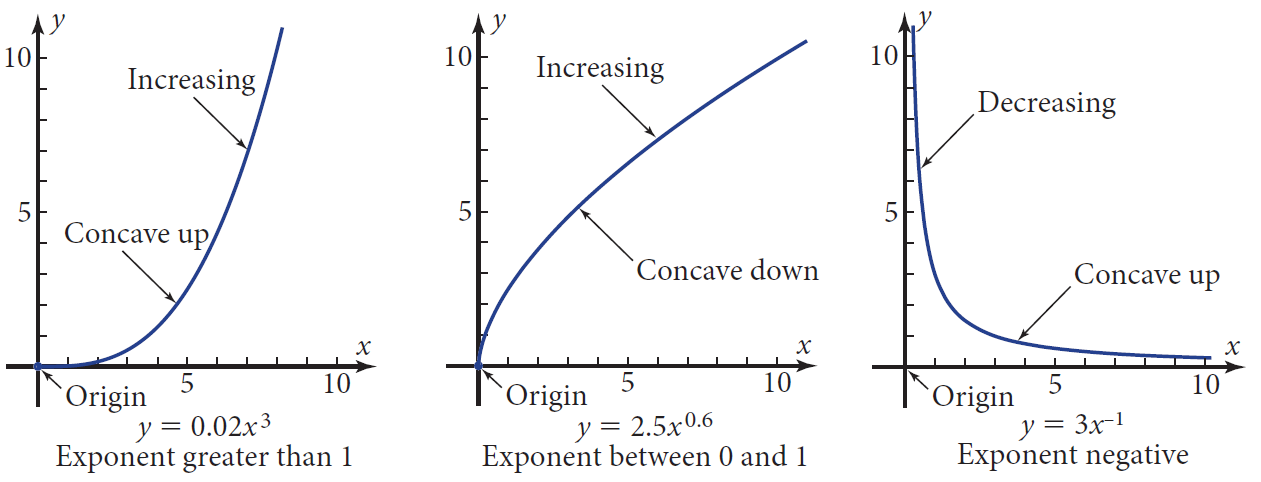
\includegraphics[width=1\textwidth]{figure/book3.png} % Adjust width here to scale the image
    \caption{Power functions}
    \label{fig:book_image3}
\end{figure}

\begin{figure}[htbp]
    \centering
    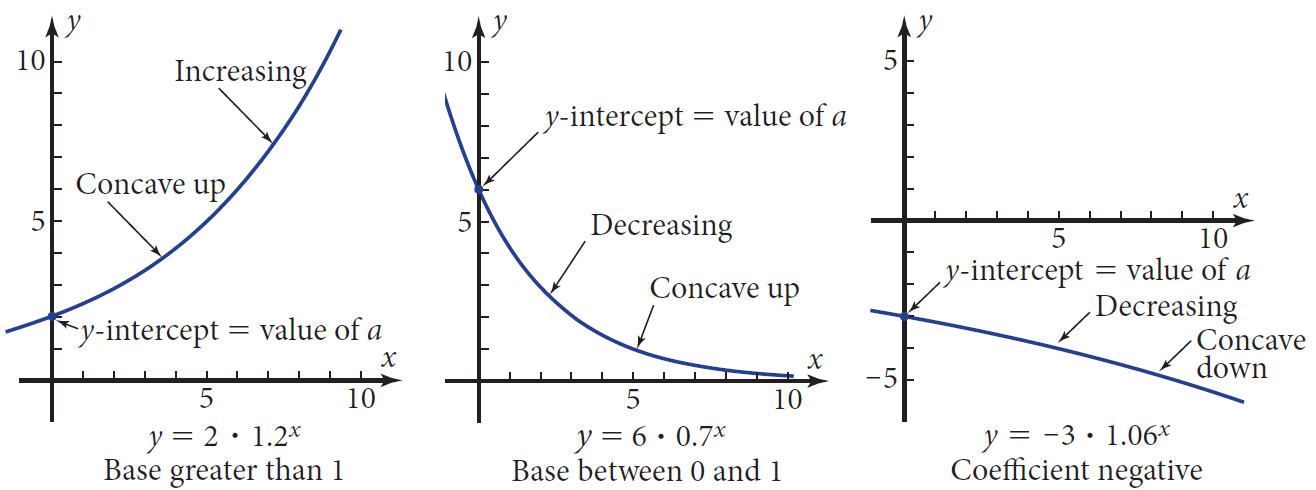
\includegraphics[width=1\textwidth]{figure/book4.png} % Adjust width here to scale the image
    \caption{Exponential functions}
    \label{fig:book_image4}
\end{figure}

\begin{definition}{Base-10 Logarithms}

\[
\log x=y \iff 10^y=x
\]

\textit{Verbally}: $\log x$ is the exponent in the power of 10 that gives $x$   
\end{definition}

\begin{custombox}{Properties of base-10 logarithms}
\begin{itemize}
    \item Log of a Product:
    
    \[
    \log x y=\log x+\log y
    \]
    
    \textit{Verbally}: The $\log$ of a product equals the sum of the logs of the factors.
    \vspace{0.2cm}
    \item Log of a Quotient:
    
    \[
    \log \frac{x}{y}=\log x-\log y
    \]
    \vspace{0.1cm}
    \textit{Verbally}: The $\log$ of a quotient equals the log of the numerator minus the $\log$ of the denominator.
    \vspace{0.2cm}
    \item Log of a Power:
    \[
    \log x^y=y \log x
    \]
    \textit{Verbally}: The $\log$ of a power equals the exponent times the log of the base.
\end{itemize}

   
\end{custombox}

\begin{definition}{Common Logarithm and Natural Logarithm}
\hspace{1cm} \textit{Common}: The symbol $\log x$ means $\log _{10} x$.

\hspace{1cm}  \textit{Natural}: \hspace{0.2cm}The symbol $\ln x$ means $\log _e x$, where $e$ is a constant equal to $2.71828182845 \ldots$
\end{definition}

\begin{custombox}{The Change-of-Base Property of Logarithms}

\begin{equation*}
\log _a x=\frac{\log _b x}{\log _b a} \quad \text { or } \quad \log _a x=\frac{1}{\log _b a}\left(\log _b x\right)
\end{equation*}
    
\end{custombox}

\begin{custombox}{Properties of Logarithms}
\setlength{\leftskip}{1cm}  % Reset the text indent
\setlength{\rightskip}{1cm} % Reset the right indent
The Logarithm of a Power:
$$
\log _b x^y=y \log _b x
$$
The Logarithm of a Product:
$$
\log _b(x y)=\log _b x+\log _b y
$$
The Logarithm of a Quotient:
$$
\log _b \frac{x}{y}=\log _b x-\log _b y
$$
\setlength{\leftskip}{0cm}  % Reset the text indent
\setlength{\rightskip}{0cm} % Reset the right indent

\end{custombox}

